% ---------------------------------------------------------------
% Generated by FlowTikZ (flowcharts and data charts to LaTeX)
% Every coordinate below is derived from the editor diagram model.
% Safe to edit by hand, but regenerating will overwrite changes.
% ---------------------------------------------------------------

\documentclass[border=8pt]{standalone}
\usepackage[T1]{fontenc}
\usepackage[utf8]{inputenc}
\usepackage{xcolor}
\usepackage{tikz}
\usepackage{pgfplots}
\pgfplotsset{compat=1.18}
\usetikzlibrary{arrows.meta}

% ---- Colour definitions ----
\definecolor{fc118DFF}{HTML}{118DFF}
\definecolor{fc12161C}{HTML}{12161C}
\definecolor{fc12239E}{HTML}{12239E}
\definecolor{fc1F2933}{HTML}{1F2933}
\definecolor{fc334F6D}{HTML}{334F6D}
\definecolor{fc4A5563}{HTML}{4A5563}
\definecolor{fc4E79A7}{HTML}{4E79A7}
\definecolor{fc8DD3C7}{HTML}{8DD3C7}
\definecolor{fc9D5C1C}{HTML}{9D5C1C}
\definecolor{fcBEBADA}{HTML}{BEBADA}
\definecolor{fcC3CCD6}{HTML}{C3CCD6}
\definecolor{fcDDE3EA}{HTML}{DDE3EA}
\definecolor{fcE15759}{HTML}{E15759}
\definecolor{fcF28E2B}{HTML}{F28E2B}
\definecolor{fcF7F9FB}{HTML}{F7F9FB}
\definecolor{fcFDB462}{HTML}{FDB462}

% ---- Style definitions ----
\tikzset{
  fcnode/.style={
    draw, inner sep=0pt, outer sep=0pt, align=center,
    line join=round, line cap=butt
  },
  fcpath/.style={line join=round, line cap=butt},
  fcedge/.style={line join=round, line cap=butt},
  fclabel/.style={inner sep=1.4pt, outer sep=0pt, align=center},
}
\tikzset{
  fctext/.style={inner sep=0pt, outer sep=0pt, align=center,
    font=\fontsize{#1pt}{#1pt}\selectfont\sffamily,
    text height={0.7*#1pt}, text depth={0.2*#1pt}},
  fctextb/.style={fctext=#1, font=\fontsize{#1pt}{#1pt}\selectfont\sffamily\bfseries},
}

\begin{document}
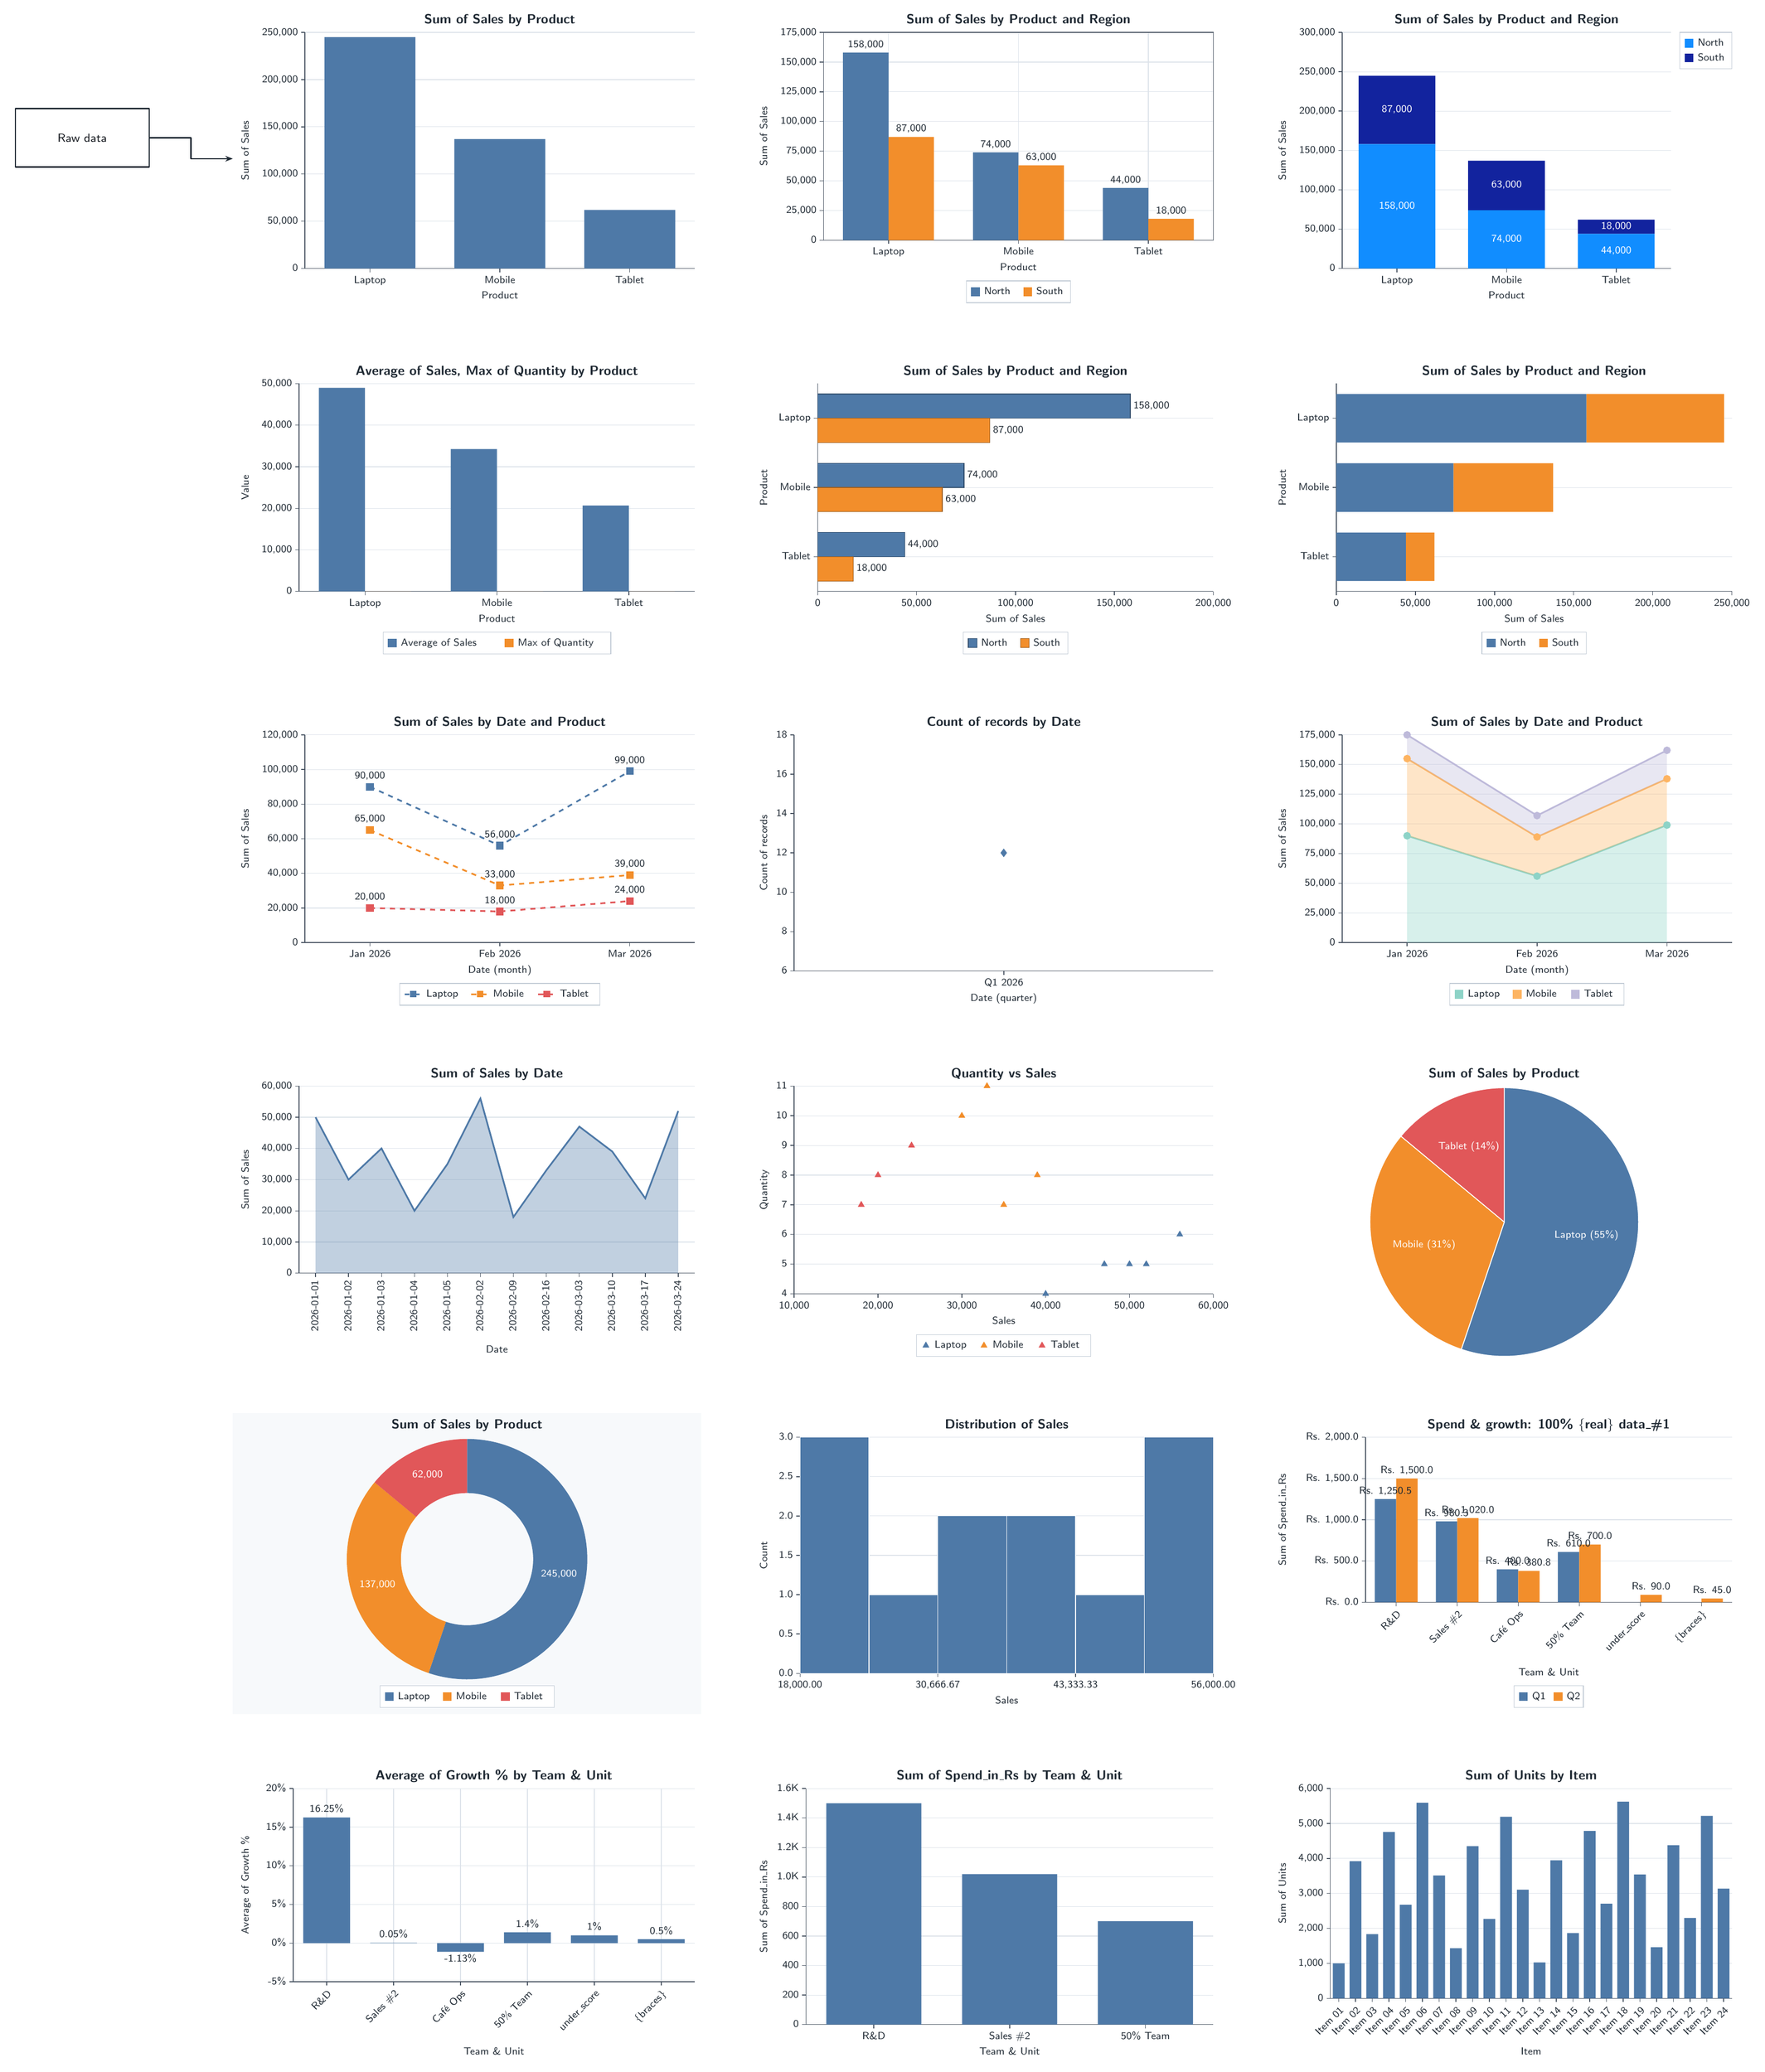
\begin{tikzpicture}[x=1cm, y=1cm]
  % ---- Nodes ----
  % c1 - Column chart "Sum of Sales by Product"
  % Data: Sample sales data (12 of 12 rows used)
  % Axis = Product; Values = Sum of Sales
  %   Product | Sum of Sales
  %   Laptop  | 245,000
  %   Mobile  | 137,000
  %   Tablet  | 62,000
  \begin{scope}
  \begin{axis}[
    name=c1axis,
    at={(7.7238cm,-8.225cm)},
    anchor=south west,
    scale only axis,
    width=9.3202cm,
    height=5.6452cm,
    xmin=-0.5,
    xmax=2.5,
    ymin=0,
    ymax=250000,
    enlargelimits=false,
    clip=false,
    scaled ticks=false,
    xtick={0,1,2},
    xticklabels={{Laptop},{Mobile},{Tablet}},
    ytick={0,50000,100000,150000,200000,250000},
    yticklabels={{0},{50,000},{100,000},{150,000},{200,000},{250,000}},
    minor tick num=0,
    tick pos=left,
    tick align=outside,
    major tick length=2.589pt,
    tick style={draw=fc4A5563, line width=0.518pt},
    axis line style={draw=fc4A5563, line width=0.518pt},
    axis x line*=bottom,
    axis y line*=left,
    tick label style={fctext=7.398, text=fc1F2933},
    xticklabel style={anchor=north, yshift=-2.219pt},
    yticklabel style={anchor=east, xshift=-2.219pt},
    ymajorgrids=true,
    major grid style={draw=fcDDE3EA, line width=0.414pt},
    title={Sum of Sales by Product},
    every axis title shift=0pt,
    title style={fctextb=8.877, text=fc1F2933, anchor=south, yshift=0pt, at={(axis description cs:0.5,1.0253)}},
    xlabel={Product},
    xlabel style={fctext=7.398, text=fc1F2933, anchor=north, at={(axis description cs:0.5,-0.0967)}},
    ylabel={Sum of Sales},
    ylabel style={fctext=7.398, text=fc1F2933, anchor=south, rotate=0, at={(axis description cs:-0.1389,0.5)}}
  ]
  % Series: Sum of Sales
  \addplot[ybar, bar width=0.7, bar shift=0, fill=fc4E79A7, draw=none]
    coordinates {
      (0,245000) % Laptop
      (1,137000) % Mobile
      (2,62000) % Tablet
    };
  \end{axis}
  \coordinate (c1) at (11.6,-5.6);
  \end{scope}
  % c2 - Column chart "Sum of Sales by Product and Region"
  % Data: Sample sales data (12 of 12 rows used)
  % Axis = Product; Values = Sum of Sales; Legend = Region
  %   Product | North   | South
  %   Laptop  | 158,000 | 87,000
  %   Mobile  | 74,000  | 63,000
  %   Tablet  | 44,000  | 18,000
  \begin{scope}
  \begin{axis}[
    name=c2axis,
    at={(20.1238cm,-7.549cm)},
    anchor=south west,
    scale only axis,
    width=9.3202cm,
    height=4.9692cm,
    xmin=-0.5,
    xmax=2.5,
    ymin=0,
    ymax=175000,
    enlargelimits=false,
    clip=false,
    scaled ticks=false,
    xtick={0,1,2},
    xticklabels={{Laptop},{Mobile},{Tablet}},
    ytick={0,25000,50000,75000,100000,125000,150000,175000},
    yticklabels={{0},{25,000},{50,000},{75,000},{100,000},{125,000},{150,000},{175,000}},
    minor tick num=0,
    tick pos=left,
    tick align=outside,
    major tick length=2.589pt,
    tick style={draw=fc4A5563, line width=0.518pt},
    axis line style={draw=fc4A5563, line width=0.518pt},
    tick label style={fctext=7.398, text=fc1F2933},
    xticklabel style={anchor=north, yshift=-2.219pt},
    yticklabel style={anchor=east, xshift=-2.219pt},
    xmajorgrids=true,
    ymajorgrids=true,
    major grid style={draw=fcDDE3EA, line width=0.414pt},
    title={Sum of Sales by Product and Region},
    every axis title shift=0pt,
    title style={fctextb=8.877, text=fc1F2933, anchor=south, yshift=0pt, at={(axis description cs:0.5,1.0288)}},
    xlabel={Product},
    xlabel style={fctext=7.398, text=fc1F2933, anchor=north, at={(axis description cs:0.5,-0.1099)}},
    ylabel={Sum of Sales},
    ylabel style={fctext=7.398, text=fc1F2933, anchor=south, rotate=0, at={(axis description cs:-0.1389,0.5)}}
  ]
  % Series: North
  \addplot[ybar, bar width=0.35, bar shift=-0.175, fill=fc4E79A7, draw=none]
    coordinates {
      (0,158000) % Laptop
      (1,74000) % Mobile
      (2,44000) % Tablet
    };
  % Series: South
  \addplot[ybar, bar width=0.35, bar shift=0.175, fill=fcF28E2B, draw=none]
    coordinates {
      (0,87000) % Laptop
      (1,63000) % Mobile
      (2,18000) % Tablet
    };
  \end{axis}
  % Data labels
  \node[fctext=6.658, text=fc1F2933, anchor=south] at (21.1335,-2.9845) {158,000};
  \node[fctext=6.658, text=fc1F2933, anchor=south] at (24.2402,-5.3697) {74,000};
  \node[fctext=6.658, text=fc1F2933, anchor=south] at (27.347,-6.2216) {44,000};
  \node[fctext=6.658, text=fc1F2933, anchor=south] at (22.2208,-5.0006) {87,000};
  \node[fctext=6.658, text=fc1F2933, anchor=south] at (25.3276,-5.6821) {63,000};
  \node[fctext=6.658, text=fc1F2933, anchor=south] at (28.4343,-6.9599) {18,000};
  % Legend
  \filldraw[fill=white, draw=fcC3CCD6, line width=0.455pt] (23.5359,-8.524) rectangle (26.0319,-9.044);
  \fill[fc4E79A7] (23.6529,-8.68) rectangle (23.8609,-8.888);
  \node[fctext=7.398, text=fc1F2933, anchor=west] at (23.9649,-8.784) {North};
  \fill[fcF28E2B] (24.9009,-8.68) rectangle (25.1089,-8.888);
  \node[fctext=7.398, text=fc1F2933, anchor=west] at (25.2129,-8.784) {South};
  \coordinate (c2) at (24,-5.6);
  \end{scope}
  % c3 - Column chart "Sum of Sales by Product and Region"
  % Data: Sample sales data (12 of 12 rows used)
  % Axis = Product; Values = Sum of Sales; Legend = Region
  %   Product | North   | South
  %   Laptop  | 158,000 | 87,000
  %   Mobile  | 74,000  | 63,000
  %   Tablet  | 44,000  | 18,000
  \begin{scope}
  \begin{axis}[
    name=c3axis,
    at={(32.5238cm,-8.225cm)},
    anchor=south west,
    scale only axis,
    width=7.8642cm,
    height=5.6452cm,
    xmin=-0.5,
    xmax=2.5,
    ymin=0,
    ymax=300000,
    enlargelimits=false,
    clip=false,
    scaled ticks=false,
    xtick={0,1,2},
    xticklabels={{Laptop},{Mobile},{Tablet}},
    ytick={0,50000,100000,150000,200000,250000,300000},
    yticklabels={{0},{50,000},{100,000},{150,000},{200,000},{250,000},{300,000}},
    minor tick num=0,
    tick pos=left,
    tick align=outside,
    major tick length=2.589pt,
    tick style={draw=fc4A5563, line width=0.518pt},
    axis line style={draw=fc4A5563, line width=0.518pt},
    axis x line*=bottom,
    axis y line*=left,
    tick label style={fctext=7.398, text=fc1F2933},
    xticklabel style={anchor=north, yshift=-2.219pt},
    yticklabel style={anchor=east, xshift=-2.219pt},
    ymajorgrids=true,
    major grid style={draw=fcDDE3EA, line width=0.414pt},
    ybar stacked,
    bar width=0.7,
    title={Sum of Sales by Product and Region},
    every axis title shift=0pt,
    title style={fctextb=8.877, text=fc1F2933, anchor=south, yshift=0pt, at={(axis description cs:0.5,1.0253)}},
    xlabel={Product},
    xlabel style={fctext=7.398, text=fc1F2933, anchor=north, at={(axis description cs:0.5,-0.0967)}},
    ylabel={Sum of Sales},
    ylabel style={fctext=7.398, text=fc1F2933, anchor=south, rotate=0, at={(axis description cs:-0.1646,0.5)}}
  ]
  % Series: North
  \addplot[fill=fc118DFF, draw=none]
    coordinates {
      (0,158000) % Laptop
      (1,74000) % Mobile
      (2,44000) % Tablet
    };
  % Series: South
  \addplot[fill=fc12239E, draw=none]
    coordinates {
      (0,87000) % Laptop
      (1,63000) % Mobile
      (2,18000) % Tablet
    };
  \end{axis}
  % Data labels
  \node[fctext=6.658, text=white, anchor=center] at (33.8345,-6.7384) {158,000};
  \node[fctext=6.658, text=white, anchor=center] at (36.4559,-7.5288) {74,000};
  \node[fctext=6.658, text=white, anchor=center] at (39.0773,-7.811) {44,000};
  \node[fctext=6.658, text=white, anchor=center] at (33.8345,-4.4333) {87,000};
  \node[fctext=6.658, text=white, anchor=center] at (36.4559,-6.2398) {63,000};
  \node[fctext=6.658, text=white, anchor=center] at (39.0773,-7.2277) {18,000};
  % Legend
  \filldraw[fill=white, draw=fcC3CCD6, line width=0.455pt] (40.596,-2.5798) rectangle (41.844,-3.4508);
  \fill[fc118DFF] (40.713,-2.7358) rectangle (40.921,-2.9438);
  \node[fctext=7.398, text=fc1F2933, anchor=west] at (41.025,-2.8398) {North};
  \fill[fc12239E] (40.713,-3.0868) rectangle (40.921,-3.2948);
  \node[fctext=7.398, text=fc1F2933, anchor=west] at (41.025,-3.1908) {South};
  \coordinate (c3) at (36.4,-5.6);
  \end{scope}
  % c4 - Column chart "Average of Sales, Max of Quantity by Product"
  % Data: Sample sales data (12 of 12 rows used)
  % Axis = Product; Values = Average of Sales, Max of Quantity
  %   Product | Average of Sales | Max of Quantity
  %   Laptop  | 49,000           | 6
  %   Mobile  | 34,250           | 11
  %   Tablet  | 20,666.6667      | 9
  \begin{scope}
  \begin{axis}[
    name=c4axis,
    at={(7.5834cm,-15.949cm)},
    anchor=south west,
    scale only axis,
    width=9.4606cm,
    height=4.9692cm,
    xmin=-0.5,
    xmax=2.5,
    ymin=0,
    ymax=50000,
    enlargelimits=false,
    clip=false,
    scaled ticks=false,
    xtick={0,1,2},
    xticklabels={{Laptop},{Mobile},{Tablet}},
    ytick={0,10000,20000,30000,40000,50000},
    yticklabels={{0},{10,000},{20,000},{30,000},{40,000},{50,000}},
    minor tick num=0,
    tick pos=left,
    tick align=outside,
    major tick length=2.589pt,
    tick style={draw=fc4A5563, line width=0.518pt},
    axis line style={draw=fc4A5563, line width=0.518pt},
    axis x line*=bottom,
    axis y line*=left,
    tick label style={fctext=7.398, text=fc1F2933},
    xticklabel style={anchor=north, yshift=-2.219pt},
    yticklabel style={anchor=east, xshift=-2.219pt},
    ymajorgrids=true,
    major grid style={draw=fcDDE3EA, line width=0.414pt},
    title={Average of Sales, Max of Quantity by Product},
    every axis title shift=0pt,
    title style={fctextb=8.877, text=fc1F2933, anchor=south, yshift=0pt, at={(axis description cs:0.5,1.0288)}},
    xlabel={Product},
    xlabel style={fctext=7.398, text=fc1F2933, anchor=north, at={(axis description cs:0.5,-0.1099)}},
    ylabel={Value},
    ylabel style={fctext=7.398, text=fc1F2933, anchor=south, rotate=0, at={(axis description cs:-0.122,0.5)}}
  ]
  % Series: Average of Sales
  \addplot[ybar, bar width=0.35, bar shift=-0.175, fill=fc4E79A7, draw=none]
    coordinates {
      (0,49000) % Laptop
      (1,34250) % Mobile
      (2,20666.666667) % Tablet
    };
  % Series: Max of Quantity
  \addplot[ybar, bar width=0.35, bar shift=0.175, fill=fcF28E2B, draw=none]
    coordinates {
      (0,6) % Laptop
      (1,11) % Mobile
      (2,9) % Tablet
    };
  \end{axis}
  % Legend
  \filldraw[fill=white, draw=fcC3CCD6, line width=0.455pt] (9.5915,-16.924) rectangle (15.0359,-17.444);
  \fill[fc4E79A7] (9.7085,-17.08) rectangle (9.9165,-17.288);
  \node[fctext=7.398, text=fc1F2933, anchor=west] at (10.0205,-17.184) {Average of Sales};
  \fill[fcF28E2B] (12.5009,-17.08) rectangle (12.7089,-17.288);
  \node[fctext=7.398, text=fc1F2933, anchor=west] at (12.8129,-17.184) {Max of Quantity};
  \coordinate (c4) at (11.6,-14);
  \end{scope}
  % c5 - Bar chart "Sum of Sales by Product and Region"
  % Data: Sample sales data (12 of 12 rows used)
  % Axis = Product; Values = Sum of Sales; Legend = Region
  %   Product | North   | South
  %   Laptop  | 158,000 | 87,000
  %   Mobile  | 74,000  | 63,000
  %   Tablet  | 44,000  | 18,000
  \begin{scope}
  \begin{axis}[
    name=c5axis,
    at={(19.9834cm,-15.949cm)},
    anchor=south west,
    scale only axis,
    width=9.4606cm,
    height=4.9692cm,
    xmin=0,
    xmax=200000,
    ymin=-0.5,
    ymax=2.5,
    enlargelimits=false,
    clip=false,
    scaled ticks=false,
    xtick={0,50000,100000,150000,200000},
    xticklabels={{0},{50,000},{100,000},{150,000},{200,000}},
    ytick={2,1,0},
    yticklabels={{Laptop},{Mobile},{Tablet}},
    minor tick num=0,
    tick pos=left,
    tick align=outside,
    major tick length=2.589pt,
    tick style={draw=fc4A5563, line width=0.518pt},
    axis line style={draw=fc4A5563, line width=0.518pt},
    axis x line*=bottom,
    axis y line*=left,
    tick label style={fctext=7.398, text=fc1F2933},
    xticklabel style={anchor=north, yshift=-2.219pt},
    yticklabel style={anchor=east, xshift=-2.219pt},
    ymajorgrids=true,
    major grid style={draw=fcDDE3EA, line width=0.414pt},
    title={Sum of Sales by Product and Region},
    every axis title shift=0pt,
    title style={fctextb=8.877, text=fc1F2933, anchor=south, yshift=0pt, at={(axis description cs:0.5,1.0288)}},
    xlabel={Sum of Sales},
    xlabel style={fctext=7.398, text=fc1F2933, anchor=north, at={(axis description cs:0.5,-0.1099)}},
    ylabel={Product},
    ylabel style={fctext=7.398, text=fc1F2933, anchor=south, rotate=0, at={(axis description cs:-0.122,0.5)}}
  ]
  % Series: North
  \addplot[xbar, bar width=0.35, bar shift=0.175, fill=fc4E79A7, draw=fc334F6D, line width=0.444pt]
    coordinates {
      (158000,2) % Laptop
      (74000,1) % Mobile
      (44000,0) % Tablet
    };
  % Series: South
  \addplot[xbar, bar width=0.35, bar shift=-0.175, fill=fcF28E2B, draw=fc9D5C1C, line width=0.444pt]
    coordinates {
      (87000,2) % Laptop
      (63000,1) % Mobile
      (18000,0) % Tablet
    };
  \end{axis}
  % Data labels
  \node[fctext=6.658, text=fc1F2933, anchor=west] at (27.5353,-11.5181) {158,000};
  \node[fctext=6.658, text=fc1F2933, anchor=west] at (23.5618,-13.1745) {74,000};
  \node[fctext=6.658, text=fc1F2933, anchor=west] at (22.1427,-14.8309) {44,000};
  \node[fctext=6.658, text=fc1F2933, anchor=west] at (24.1768,-12.0979) {87,000};
  \node[fctext=6.658, text=fc1F2933, anchor=west] at (23.0415,-13.7543) {63,000};
  \node[fctext=6.658, text=fc1F2933, anchor=west] at (20.9129,-15.4107) {18,000};
  % Legend
  \filldraw[fill=white, draw=fcC3CCD6, line width=0.455pt] (23.4657,-16.924) rectangle (25.9617,-17.444);
  \filldraw[fill=fc4E79A7, draw=fc334F6D, line width=0.455pt] (23.5827,-17.08) rectangle (23.7907,-17.288);
  \node[fctext=7.398, text=fc1F2933, anchor=west] at (23.8947,-17.184) {North};
  \filldraw[fill=fcF28E2B, draw=fc9D5C1C, line width=0.455pt] (24.8307,-17.08) rectangle (25.0387,-17.288);
  \node[fctext=7.398, text=fc1F2933, anchor=west] at (25.1427,-17.184) {South};
  \coordinate (c5) at (24,-14);
  \end{scope}
  % c6 - Bar chart "Sum of Sales by Product and Region"
  % Data: Sample sales data (12 of 12 rows used)
  % Axis = Product; Values = Sum of Sales; Legend = Region
  %   Product | North   | South
  %   Laptop  | 158,000 | 87,000
  %   Mobile  | 74,000  | 63,000
  %   Tablet  | 44,000  | 18,000
  \begin{scope}
  \begin{axis}[
    name=c6axis,
    at={(32.3834cm,-15.949cm)},
    anchor=south west,
    scale only axis,
    width=9.4606cm,
    height=4.9692cm,
    xmin=0,
    xmax=250000,
    ymin=-0.5,
    ymax=2.5,
    enlargelimits=false,
    clip=false,
    scaled ticks=false,
    xtick={0,50000,100000,150000,200000,250000},
    xticklabels={{0},{50,000},{100,000},{150,000},{200,000},{250,000}},
    ytick={2,1,0},
    yticklabels={{Laptop},{Mobile},{Tablet}},
    minor tick num=0,
    tick pos=left,
    tick align=outside,
    major tick length=2.589pt,
    tick style={draw=fc4A5563, line width=0.518pt},
    axis line style={draw=fc4A5563, line width=0.518pt},
    axis x line*=bottom,
    axis y line*=left,
    tick label style={fctext=7.398, text=fc1F2933},
    xticklabel style={anchor=north, yshift=-2.219pt},
    yticklabel style={anchor=east, xshift=-2.219pt},
    ymajorgrids=true,
    major grid style={draw=fcDDE3EA, line width=0.414pt},
    xbar stacked,
    bar width=0.7,
    title={Sum of Sales by Product and Region},
    every axis title shift=0pt,
    title style={fctextb=8.877, text=fc1F2933, anchor=south, yshift=0pt, at={(axis description cs:0.5,1.0288)}},
    xlabel={Sum of Sales},
    xlabel style={fctext=7.398, text=fc1F2933, anchor=north, at={(axis description cs:0.5,-0.1099)}},
    ylabel={Product},
    ylabel style={fctext=7.398, text=fc1F2933, anchor=south, rotate=0, at={(axis description cs:-0.122,0.5)}}
  ]
  % Series: North
  \addplot[fill=fc4E79A7, draw=none]
    coordinates {
      (158000,2) % Laptop
      (74000,1) % Mobile
      (44000,0) % Tablet
    };
  % Series: South
  \addplot[fill=fcF28E2B, draw=none]
    coordinates {
      (87000,2) % Laptop
      (63000,1) % Mobile
      (18000,0) % Tablet
    };
  \end{axis}
  % Legend
  \filldraw[fill=white, draw=fcC3CCD6, line width=0.455pt] (35.8657,-16.924) rectangle (38.3617,-17.444);
  \fill[fc4E79A7] (35.9827,-17.08) rectangle (36.1907,-17.288);
  \node[fctext=7.398, text=fc1F2933, anchor=west] at (36.2947,-17.184) {North};
  \fill[fcF28E2B] (37.2307,-17.08) rectangle (37.4387,-17.288);
  \node[fctext=7.398, text=fc1F2933, anchor=west] at (37.5427,-17.184) {South};
  \coordinate (c6) at (36.4,-14);
  \end{scope}
  % c7 - Line chart "Sum of Sales by Date and Product"
  % Data: Sample sales data (12 of 12 rows used)
  % Axis = Date; Values = Sum of Sales; Legend = Product
  %   Date     | Laptop | Mobile | Tablet
  %   Jan 2026 | 90,000 | 65,000 | 20,000
  %   Feb 2026 | 56,000 | 33,000 | 18,000
  %   Mar 2026 | 99,000 | 39,000 | 24,000
  \begin{scope}
  \begin{axis}[
    name=c7axis,
    at={(7.7238cm,-24.349cm)},
    anchor=south west,
    scale only axis,
    width=9.3202cm,
    height=4.9692cm,
    xmin=-0.5,
    xmax=2.5,
    ymin=0,
    ymax=120000,
    enlargelimits=false,
    clip=false,
    scaled ticks=false,
    xtick={0,1,2},
    xticklabels={{Jan 2026},{Feb 2026},{Mar 2026}},
    ytick={0,20000,40000,60000,80000,100000,120000},
    yticklabels={{0},{20,000},{40,000},{60,000},{80,000},{100,000},{120,000}},
    minor tick num=0,
    tick pos=left,
    tick align=outside,
    major tick length=2.589pt,
    tick style={draw=fc4A5563, line width=0.518pt},
    axis line style={draw=fc4A5563, line width=0.518pt},
    axis x line*=bottom,
    axis y line*=left,
    tick label style={fctext=7.398, text=fc1F2933},
    xticklabel style={anchor=north, yshift=-2.219pt},
    yticklabel style={anchor=east, xshift=-2.219pt},
    ymajorgrids=true,
    major grid style={draw=fcDDE3EA, line width=0.414pt},
    title={Sum of Sales by Date and Product},
    every axis title shift=0pt,
    title style={fctextb=8.877, text=fc1F2933, anchor=south, yshift=0pt, at={(axis description cs:0.5,1.0288)}},
    xlabel={Date (month)},
    xlabel style={fctext=7.398, text=fc1F2933, anchor=north, at={(axis description cs:0.5,-0.1099)}},
    ylabel={Sum of Sales},
    ylabel style={fctext=7.398, text=fc1F2933, anchor=south, rotate=0, at={(axis description cs:-0.1389,0.5)}}
  ]
  % Series: Laptop
  \addplot[fc4E79A7, line width=1.138pt, dash pattern=on 3.414pt off 3.414pt, mark=square*, mark size=1.992pt, mark options={solid, fill=fc4E79A7}]
    coordinates {
      (0,90000) % Jan 2026
      (1,56000) % Feb 2026
      (2,99000) % Mar 2026
    };
  % Series: Mobile
  \addplot[fcF28E2B, line width=1.138pt, dash pattern=on 3.414pt off 3.414pt, mark=square*, mark size=1.992pt, mark options={solid, fill=fcF28E2B}]
    coordinates {
      (0,65000) % Jan 2026
      (1,33000) % Feb 2026
      (2,39000) % Mar 2026
    };
  % Series: Tablet
  \addplot[fcE15759, line width=1.138pt, dash pattern=on 3.414pt off 3.414pt, mark=square*, mark size=1.992pt, mark options={solid, fill=fcE15759}]
    coordinates {
      (0,20000) % Jan 2026
      (1,18000) % Feb 2026
      (2,24000) % Mar 2026
    };
  \end{axis}
  % Data labels
  \node[fctext=6.658, text=fc1F2933, anchor=south] at (9.2772,-20.4741) {90,000};
  \node[fctext=6.658, text=fc1F2933, anchor=south] at (12.3839,-21.882) {56,000};
  \node[fctext=6.658, text=fc1F2933, anchor=south] at (15.4906,-20.1014) {99,000};
  \node[fctext=6.658, text=fc1F2933, anchor=south] at (9.2772,-21.5093) {65,000};
  \node[fctext=6.658, text=fc1F2933, anchor=south] at (12.3839,-22.8345) {33,000};
  \node[fctext=6.658, text=fc1F2933, anchor=south] at (15.4906,-22.586) {39,000};
  \node[fctext=6.658, text=fc1F2933, anchor=south] at (9.2772,-23.3728) {20,000};
  \node[fctext=6.658, text=fc1F2933, anchor=south] at (12.3839,-23.4556) {18,000};
  \node[fctext=6.658, text=fc1F2933, anchor=south] at (15.4906,-23.2072) {24,000};
  % Legend
  \filldraw[fill=white, draw=fcC3CCD6, line width=0.455pt] (9.9893,-25.324) rectangle (14.7785,-25.844);
  \draw[fc4E79A7, line width=1.138pt, dash pattern=on 3.414pt off 3.414pt] (10.1063,-25.584) -- (10.5223,-25.584);
  \path plot[mark=square*, mark size=1.992pt, mark options={solid, draw=fc4E79A7, fill=fc4E79A7}] coordinates {(10.3143,-25.584)};
  \node[fctext=7.398, text=fc1F2933, anchor=west] at (10.6263,-25.584) {Laptop};
  \draw[fcF28E2B, line width=1.138pt, dash pattern=on 3.414pt off 3.414pt] (11.7027,-25.584) -- (12.1187,-25.584);
  \path plot[mark=square*, mark size=1.992pt, mark options={solid, draw=fcF28E2B, fill=fcF28E2B}] coordinates {(11.9107,-25.584)};
  \node[fctext=7.398, text=fc1F2933, anchor=west] at (12.2227,-25.584) {Mobile};
  \draw[fcE15759, line width=1.138pt, dash pattern=on 3.414pt off 3.414pt] (13.2991,-25.584) -- (13.7151,-25.584);
  \path plot[mark=square*, mark size=1.992pt, mark options={solid, draw=fcE15759, fill=fcE15759}] coordinates {(13.5071,-25.584)};
  \node[fctext=7.398, text=fc1F2933, anchor=west] at (13.8191,-25.584) {Tablet};
  \coordinate (c7) at (11.6,-22.4);
  \end{scope}
  % c8 - Line chart "Count of records by Date"
  % Data: Sample sales data (12 of 12 rows used)
  % Axis = Date; Values = Count of records
  %   Date    | Count of records
  %   Q1 2026 | 12
  \begin{scope}
  \begin{axis}[
    name=c8axis,
    at={(19.4218cm,-25.025cm)},
    anchor=south west,
    scale only axis,
    width=10.0222cm,
    height=5.6452cm,
    xmin=-0.5,
    xmax=0.5,
    ymin=6,
    ymax=18,
    enlargelimits=false,
    clip=false,
    scaled ticks=false,
    xtick={0},
    xticklabels={{Q1 2026}},
    ytick={6,8,10,12,14,16,18},
    yticklabels={{6},{8},{10},{12},{14},{16},{18}},
    minor tick num=0,
    tick pos=left,
    tick align=outside,
    major tick length=2.589pt,
    tick style={draw=fc4A5563, line width=0.518pt},
    axis line style={draw=fc4A5563, line width=0.518pt},
    axis x line*=bottom,
    axis y line*=left,
    tick label style={fctext=7.398, text=fc1F2933},
    xticklabel style={anchor=north, yshift=-2.219pt},
    yticklabel style={anchor=east, xshift=-2.219pt},
    title={Count of records by Date},
    every axis title shift=0pt,
    title style={fctextb=8.877, text=fc1F2933, anchor=south, yshift=0pt, at={(axis description cs:0.5,1.0253)}},
    xlabel={Date (quarter)},
    xlabel style={fctext=7.398, text=fc1F2933, anchor=north, at={(axis description cs:0.5,-0.0967)}},
    ylabel={Count of records},
    ylabel style={fctext=7.398, text=fc1F2933, anchor=south, rotate=0, at={(axis description cs:-0.0591,0.5)}}
  ]
  % Series: Count of records
  \addplot[fc4E79A7, line width=1.138pt, line cap=round, dash pattern=on 0pt off 2.959pt, mark=diamond*, mark size=1.992pt, mark options={solid, fill=fc4E79A7}]
    coordinates {
      (0,12) % Q1 2026
    };
  \end{axis}
  \coordinate (c8) at (24,-22.4);
  \end{scope}
  % c9 - Area chart "Sum of Sales by Date and Product"
  % Data: Sample sales data (12 of 12 rows used)
  % Axis = Date; Values = Sum of Sales; Legend = Product
  %   Date     | Laptop | Mobile | Tablet
  %   Jan 2026 | 90,000 | 65,000 | 20,000
  %   Feb 2026 | 56,000 | 33,000 | 18,000
  %   Mar 2026 | 99,000 | 39,000 | 24,000
  \begin{scope}
  \begin{axis}[
    name=c9axis,
    at={(32.5238cm,-24.349cm)},
    anchor=south west,
    scale only axis,
    width=9.3202cm,
    height=4.9692cm,
    xmin=-0.5,
    xmax=2.5,
    ymin=0,
    ymax=175000,
    enlargelimits=false,
    clip=false,
    scaled ticks=false,
    xtick={0,1,2},
    xticklabels={{Jan 2026},{Feb 2026},{Mar 2026}},
    ytick={0,25000,50000,75000,100000,125000,150000,175000},
    yticklabels={{0},{25,000},{50,000},{75,000},{100,000},{125,000},{150,000},{175,000}},
    minor tick num=0,
    tick pos=left,
    tick align=outside,
    major tick length=2.589pt,
    tick style={draw=fc4A5563, line width=0.518pt},
    axis line style={draw=fc4A5563, line width=0.518pt},
    axis x line*=bottom,
    axis y line*=left,
    tick label style={fctext=7.398, text=fc1F2933},
    xticklabel style={anchor=north, yshift=-2.219pt},
    yticklabel style={anchor=east, xshift=-2.219pt},
    ymajorgrids=true,
    major grid style={draw=fcDDE3EA, line width=0.414pt},
    title={Sum of Sales by Date and Product},
    every axis title shift=0pt,
    title style={fctextb=8.877, text=fc1F2933, anchor=south, yshift=0pt, at={(axis description cs:0.5,1.0288)}},
    xlabel={Date (month)},
    xlabel style={fctext=7.398, text=fc1F2933, anchor=north, at={(axis description cs:0.5,-0.1099)}},
    ylabel={Sum of Sales},
    ylabel style={fctext=7.398, text=fc1F2933, anchor=south, rotate=0, at={(axis description cs:-0.1389,0.5)}}
  ]
  % Series: Laptop
  \addplot[fill=fc8DD3C7, draw=none, forget plot, fill opacity=0.35]
    coordinates {
      (0,90000) % Jan 2026 (stacked)
      (1,56000) % Feb 2026 (stacked)
      (2,99000) % Mar 2026 (stacked)
      (2,0) % Mar 2026 base
      (1,0) % Feb 2026 base
      (0,0) % Jan 2026 base
    } -- cycle;
  \addplot[fc8DD3C7, line width=1.138pt, mark=*, mark size=1.992pt, mark options={solid, fill=fc8DD3C7}]
    coordinates {
      (0,90000) % Jan 2026
      (1,56000) % Feb 2026
      (2,99000) % Mar 2026
    };
  % Series: Mobile
  \addplot[fill=fcFDB462, draw=none, forget plot, fill opacity=0.35]
    coordinates {
      (0,155000) % Jan 2026 (stacked)
      (1,89000) % Feb 2026 (stacked)
      (2,138000) % Mar 2026 (stacked)
      (2,99000) % Mar 2026 base
      (1,56000) % Feb 2026 base
      (0,90000) % Jan 2026 base
    } -- cycle;
  \addplot[fcFDB462, line width=1.138pt, mark=*, mark size=1.992pt, mark options={solid, fill=fcFDB462}]
    coordinates {
      (0,155000) % Jan 2026
      (1,89000) % Feb 2026
      (2,138000) % Mar 2026
    };
  % Series: Tablet
  \addplot[fill=fcBEBADA, draw=none, forget plot, fill opacity=0.35]
    coordinates {
      (0,175000) % Jan 2026 (stacked)
      (1,107000) % Feb 2026 (stacked)
      (2,162000) % Mar 2026 (stacked)
      (2,138000) % Mar 2026 base
      (1,89000) % Feb 2026 base
      (0,155000) % Jan 2026 base
    } -- cycle;
  \addplot[fcBEBADA, line width=1.138pt, mark=*, mark size=1.992pt, mark options={solid, fill=fcBEBADA}]
    coordinates {
      (0,175000) % Jan 2026
      (1,107000) % Feb 2026
      (2,162000) % Mar 2026
    };
  \end{axis}
  % Legend
  \filldraw[fill=white, draw=fcC3CCD6, line width=0.455pt] (35.1013,-25.324) rectangle (39.2665,-25.844);
  \fill[fc8DD3C7] (35.2183,-25.48) rectangle (35.4263,-25.688);
  \node[fctext=7.398, text=fc1F2933, anchor=west] at (35.5303,-25.584) {Laptop};
  \fill[fcFDB462] (36.6067,-25.48) rectangle (36.8147,-25.688);
  \node[fctext=7.398, text=fc1F2933, anchor=west] at (36.9187,-25.584) {Mobile};
  \fill[fcBEBADA] (37.9951,-25.48) rectangle (38.2031,-25.688);
  \node[fctext=7.398, text=fc1F2933, anchor=west] at (38.3071,-25.584) {Tablet};
  \coordinate (c9) at (36.4,-22.4);
  \end{scope}
  % c10 - Area chart "Sum of Sales by Date"
  % Data: Sample sales data (12 of 12 rows used)
  % Axis = Date; Values = Sum of Sales
  %   Date       | Sum of Sales
  %   2026-01-01 | 50,000
  %   2026-01-02 | 30,000
  %   2026-01-03 | 40,000
  %   2026-01-04 | 20,000
  %   2026-01-05 | 35,000
  %   2026-02-02 | 56,000
  %   2026-02-09 | 18,000
  %   2026-02-16 | 33,000
  %   2026-03-03 | 47,000
  %   2026-03-10 | 39,000
  %   2026-03-17 | 24,000
  %   2026-03-24 | 52,000
  \begin{scope}
  \begin{axis}[
    name=c10axis,
    at={(7.5834cm,-32.255cm)},
    anchor=south west,
    scale only axis,
    width=9.4606cm,
    height=4.4752cm,
    xmin=-0.5,
    xmax=11.5,
    ymin=0,
    ymax=60000,
    enlargelimits=false,
    clip=false,
    scaled ticks=false,
    xtick={0,1,2,3,4,5,6,7,8,9,10,11},
    xticklabels={{2026-01-01},{2026-01-02},{2026-01-03},{2026-01-04},{2026-01-05},{2026-02-02},{2026-02-09},{2026-02-16},{2026-03-03},{2026-03-10},{2026-03-17},{2026-03-24}},
    ytick={0,10000,20000,30000,40000,50000,60000},
    yticklabels={{0},{10,000},{20,000},{30,000},{40,000},{50,000},{60,000}},
    minor tick num=0,
    tick pos=left,
    tick align=outside,
    major tick length=2.589pt,
    tick style={draw=fc4A5563, line width=0.518pt},
    axis line style={draw=fc4A5563, line width=0.518pt},
    axis x line*=bottom,
    axis y line*=left,
    tick label style={fctext=7.398, text=fc1F2933},
    xticklabel style={anchor=east, yshift=-2.219pt, rotate=90},
    yticklabel style={anchor=east, xshift=-2.219pt},
    ymajorgrids=true,
    major grid style={draw=fcDDE3EA, line width=0.414pt},
    title={Sum of Sales by Date},
    every axis title shift=0pt,
    title style={fctextb=8.877, text=fc1F2933, anchor=south, yshift=0pt, at={(axis description cs:0.5,1.032)}},
    xlabel={Date},
    xlabel style={fctext=7.398, text=fc1F2933, anchor=north, at={(axis description cs:0.5,-0.3834)}},
    ylabel={Sum of Sales},
    ylabel style={fctext=7.398, text=fc1F2933, anchor=south, rotate=0, at={(axis description cs:-0.122,0.5)}}
  ]
  % Series: Sum of Sales
  \addplot[fill=fc4E79A7, draw=none, forget plot, fill opacity=0.35]
    coordinates {
      (0,50000) % 2026-01-01
      (1,30000) % 2026-01-02
      (2,40000) % 2026-01-03
      (3,20000) % 2026-01-04
      (4,35000) % 2026-01-05
      (5,56000) % 2026-02-02
      (6,18000) % 2026-02-09
      (7,33000) % 2026-02-16
      (8,47000) % 2026-03-03
      (9,39000) % 2026-03-10
      (10,24000) % 2026-03-17
      (11,52000) % 2026-03-24
      (11,0) % 2026-03-24 base
      (10,0) % 2026-03-17 base
      (9,0) % 2026-03-10 base
      (8,0) % 2026-03-03 base
      (7,0) % 2026-02-16 base
      (6,0) % 2026-02-09 base
      (5,0) % 2026-02-02 base
      (4,0) % 2026-01-05 base
      (3,0) % 2026-01-04 base
      (2,0) % 2026-01-03 base
      (1,0) % 2026-01-02 base
      (0,0) % 2026-01-01 base
    } -- cycle;
  \addplot[fc4E79A7, line width=1.138pt, mark=none]
    coordinates {
      (0,50000) % 2026-01-01
      (1,30000) % 2026-01-02
      (2,40000) % 2026-01-03
      (3,20000) % 2026-01-04
      (4,35000) % 2026-01-05
      (5,56000) % 2026-02-02
      (6,18000) % 2026-02-09
      (7,33000) % 2026-02-16
      (8,47000) % 2026-03-03
      (9,39000) % 2026-03-10
      (10,24000) % 2026-03-17
      (11,52000) % 2026-03-24
    };
  \end{axis}
  \coordinate (c10) at (11.6,-30.8);
  \end{scope}
  % c11 - Scatter chart "Quantity vs Sales"
  % Data: Sample sales data (12 of 12 rows used)
  % X = Sales; Y = Quantity; Legend = Product
  \begin{scope}
  \begin{axis}[
    name=c11axis,
    at={(19.4218cm,-32.749cm)},
    anchor=south west,
    scale only axis,
    width=10.0222cm,
    height=4.9692cm,
    xmin=10000,
    xmax=60000,
    ymin=4,
    ymax=11,
    enlargelimits=false,
    clip=false,
    scaled ticks=false,
    xtick={10000,20000,30000,40000,50000,60000},
    xticklabels={{10,000},{20,000},{30,000},{40,000},{50,000},{60,000}},
    ytick={4,5,6,7,8,9,10,11},
    yticklabels={{4},{5},{6},{7},{8},{9},{10},{11}},
    minor tick num=0,
    tick pos=left,
    tick align=outside,
    major tick length=2.589pt,
    tick style={draw=fc4A5563, line width=0.518pt},
    axis line style={draw=fc4A5563, line width=0.518pt},
    axis x line*=bottom,
    axis y line*=left,
    tick label style={fctext=7.398, text=fc1F2933},
    xticklabel style={anchor=north, yshift=-2.219pt},
    yticklabel style={anchor=east, xshift=-2.219pt},
    ymajorgrids=true,
    major grid style={draw=fcDDE3EA, line width=0.414pt},
    title={Quantity vs Sales},
    every axis title shift=0pt,
    title style={fctextb=8.877, text=fc1F2933, anchor=south, yshift=0pt, at={(axis description cs:0.5,1.0288)}},
    xlabel={Sales},
    xlabel style={fctext=7.398, text=fc1F2933, anchor=north, at={(axis description cs:0.5,-0.1099)}},
    ylabel={Quantity},
    ylabel style={fctext=7.398, text=fc1F2933, anchor=south, rotate=0, at={(axis description cs:-0.0591,0.5)}}
  ]
  % Series: Laptop
  \addplot[only marks, mark=triangle*, mark size=2.276pt, mark options={draw=fc4E79A7, fill=fc4E79A7}]
    coordinates {
      (50000,5) % 50000, 5
      (40000,4) % 40000, 4
      (56000,6) % 56000, 6
      (47000,5) % 47000, 5
      (52000,5) % 52000, 5
    };
  % Series: Mobile
  \addplot[only marks, mark=triangle*, mark size=2.276pt, mark options={draw=fcF28E2B, fill=fcF28E2B}]
    coordinates {
      (30000,10) % 30000, 10
      (35000,7) % 35000, 7
      (33000,11) % 33000, 11
      (39000,8) % 39000, 8
    };
  % Series: Tablet
  \addplot[only marks, mark=triangle*, mark size=2.276pt, mark options={draw=fcE15759, fill=fcE15759}]
    coordinates {
      (20000,8) % 20000, 8
      (18000,7) % 18000, 7
      (24000,9) % 24000, 9
    };
  \end{axis}
  % Legend
  \filldraw[fill=white, draw=fcC3CCD6, line width=0.455pt] (22.3503,-33.724) rectangle (26.5155,-34.244);
  \path plot[mark=triangle*, mark size=2.276pt, mark options={solid, draw=fc4E79A7, fill=fc4E79A7}] coordinates {(22.5713,-33.984)};
  \node[fctext=7.398, text=fc1F2933, anchor=west] at (22.7793,-33.984) {Laptop};
  \path plot[mark=triangle*, mark size=2.276pt, mark options={solid, draw=fcF28E2B, fill=fcF28E2B}] coordinates {(23.9597,-33.984)};
  \node[fctext=7.398, text=fc1F2933, anchor=west] at (24.1677,-33.984) {Mobile};
  \path plot[mark=triangle*, mark size=2.276pt, mark options={solid, draw=fcE15759, fill=fcE15759}] coordinates {(25.3481,-33.984)};
  \node[fctext=7.398, text=fc1F2933, anchor=west] at (25.5561,-33.984) {Tablet};
  \coordinate (c11) at (24,-30.8);
  \end{scope}
  % c12 - Pie chart "Sum of Sales by Product"
  % Data: Sample sales data (12 of 12 rows used)
  % Axis = Product; Values = Sum of Sales
  %   Product | Sum of Sales
  %   Laptop  | 245,000
  %   Mobile  | 137,000
  %   Tablet  | 62,000
  \begin{scope}
  \node[fctextb=8.877, text=fc1F2933, anchor=north] at (36.4,-27.356) {Sum of Sales by Product};
  % Laptop: 245000
  \filldraw[fill=fc4E79A7, draw=white, line width=0.592pt] (36.4,-31.0314) -- (36.4,-27.8188) arc[start angle=90, end angle=-108.6486, radius=3.2126cm] -- cycle;
  % Mobile: 137000
  \filldraw[fill=fcF28E2B, draw=white, line width=0.592pt] (36.4,-31.0314) -- (35.3727,-34.0753) arc[start angle=-108.6486, end angle=-219.7297, radius=3.2126cm] -- cycle;
  % Tablet: 62000
  \filldraw[fill=fcE15759, draw=white, line width=0.592pt] (36.4,-31.0314) -- (33.9293,-28.978) arc[start angle=-219.7297, end angle=-270, radius=3.2126cm] -- cycle;
  % Slice labels
  \node[fctext=7.398, text=white, anchor=center] at (38.3655,-31.3541) {Laptop (55\%)};
  \node[fctext=7.398, text=white, anchor=center] at (34.4835,-31.5741) {Mobile (31\%)};
  \node[fctext=7.398, text=white, anchor=center] at (35.554,-29.2282) {Tablet (14\%)};
  \coordinate (c12) at (36.4,-30.8);
  \end{scope}
  % c13 - Donut chart "Sum of Sales by Product"
  % Data: Sample sales data (12 of 12 rows used)
  % Axis = Product; Values = Sum of Sales
  %   Product | Sum of Sales
  %   Laptop  | 245,000
  %   Mobile  | 137,000
  %   Tablet  | 62,000
  \begin{scope}
  \fill[fcF7F9FB] (6,-35.6) rectangle (17.2,-42.8);
  \node[fctextb=8.877, text=fc1F2933, anchor=north] at (11.6,-35.756) {Sum of Sales by Product};
  % Laptop: 245000
  \fill[fc4E79A7] (11.6,-36.2188) arc[start angle=90, end angle=-108.6486, radius=2.8746cm] -- (11.0944,-40.5914) arc[start angle=-108.6486, end angle=90, radius=1.581cm] -- cycle;
  % Mobile: 137000
  \fill[fcF28E2B] (10.6808,-41.8171) arc[start angle=-108.6486, end angle=-219.7297, radius=2.8746cm] -- (10.3841,-38.0829) arc[start angle=-219.7297, end angle=-108.6486, radius=1.581cm] -- cycle;
  % Tablet: 62000
  \fill[fcE15759] (9.3892,-37.2561) arc[start angle=-219.7297, end angle=-270, radius=2.8746cm] -- (11.6,-37.5124) arc[start angle=-270, end angle=-219.7297, radius=1.581cm] -- cycle;
  % Slice labels
  \node[fctext=7.398, text=white, anchor=center] at (13.7984,-39.4544) {245,000};
  \node[fctext=7.398, text=white, anchor=center] at (9.4565,-39.7004) {137,000};
  \node[fctext=7.398, text=white, anchor=center] at (10.6537,-37.0765) {62,000};
  % Legend
  \filldraw[fill=white, draw=fcC3CCD6, line width=0.455pt] (9.5174,-42.124) rectangle (13.6826,-42.644);
  \fill[fc4E79A7] (9.6344,-42.28) rectangle (9.8424,-42.488);
  \node[fctext=7.398, text=fc1F2933, anchor=west] at (9.9464,-42.384) {Laptop};
  \fill[fcF28E2B] (11.0228,-42.28) rectangle (11.2308,-42.488);
  \node[fctext=7.398, text=fc1F2933, anchor=west] at (11.3348,-42.384) {Mobile};
  \fill[fcE15759] (12.4112,-42.28) rectangle (12.6192,-42.488);
  \node[fctext=7.398, text=fc1F2933, anchor=west] at (12.7232,-42.384) {Tablet};
  \coordinate (c13) at (11.6,-39.2);
  \end{scope}
  % c14 - Histogram chart "Distribution of Sales"
  % Data: Sample sales data (12 of 12 rows used)
  % Field = Sales
  \begin{scope}
  \begin{axis}[
    name=c14axis,
    at={(19.5622cm,-41.825cm)},
    anchor=south west,
    scale only axis,
    width=9.8818cm,
    height=5.6452cm,
    xmin=18000,
    xmax=56000,
    ymin=0,
    ymax=3,
    enlargelimits=false,
    clip=false,
    scaled ticks=false,
    xtick={18000,30666.666667,43333.333333,56000},
    xticklabels={{18,000.00},{30,666.67},{43,333.33},{56,000.00}},
    ytick={0,0.5,1,1.5,2,2.5,3},
    yticklabels={{0.0},{0.5},{1.0},{1.5},{2.0},{2.5},{3.0}},
    minor tick num=0,
    tick pos=left,
    tick align=outside,
    major tick length=2.589pt,
    tick style={draw=fc4A5563, line width=0.518pt},
    axis line style={draw=fc4A5563, line width=0.518pt},
    axis x line*=bottom,
    axis y line*=left,
    tick label style={fctext=7.398, text=fc1F2933},
    xticklabel style={anchor=north, yshift=-2.219pt},
    yticklabel style={anchor=east, xshift=-2.219pt},
    ymajorgrids=true,
    major grid style={draw=fcDDE3EA, line width=0.414pt},
    title={Distribution of Sales},
    every axis title shift=0pt,
    title style={fctextb=8.877, text=fc1F2933, anchor=south, yshift=0pt, at={(axis description cs:0.5,1.0253)}},
    xlabel={Sales},
    xlabel style={fctext=7.398, text=fc1F2933, anchor=north, at={(axis description cs:0.5,-0.0967)}},
    ylabel={Count},
    ylabel style={fctext=7.398, text=fc1F2933, anchor=south, rotate=0, at={(axis description cs:-0.0742,0.5)}}
  ]
  % Series: Count
  \addplot[ybar, bar width=6333.3333, bar shift=0, fill=fc4E79A7, draw=white, line width=0.444pt]
    coordinates {
      (21166.666667,3) % 18000 to 24333.333333333
      (27500,1) % 24333.333333333 to 30666.666666667
      (33833.333333,2) % 30666.666666667 to 37000
      (40166.666667,2) % 37000 to 43333.333333333
      (46500,1) % 43333.333333333 to 49666.666666667
      (52833.333333,3) % 49666.666666667 to 56000
    };
  \end{axis}
  \coordinate (c14) at (24,-39.2);
  \end{scope}
  % c15 - Column chart "Spend & growth: 100\% {real} data_#1"
  % Data: R&D budget_2026 (50\% split) #1 (10 of 10 rows used)
  % Axis = Team & Unit; Values = Sum of Spend_in_Rs; Legend = Quarter
  %   Team & Unit | Q1      | Q2
  %   R&D         | 1,250.5 | 1,500.0
  %   Sales #2    | 980.3   | 1,020.0
  %   Café Ops    | 400.0   | 380.8
  %   50\% Team    | 610.0   | 700.0
  %   under_score | -       | 90.0
  %   {braces}    | -       | 45.0
  \begin{scope}
  \begin{axis}[
    name=c15axis,
    at={(33.0854cm,-40.1255cm)},
    anchor=south west,
    scale only axis,
    width=8.7586cm,
    height=3.9457cm,
    xmin=-0.5,
    xmax=5.5,
    ymin=0,
    ymax=2000,
    enlargelimits=false,
    clip=false,
    scaled ticks=false,
    xtick={0,1,2,3,4,5},
    xticklabels={{R\&D},{Sales \#2},{Café Ops},{50\% Team},{under\_score},{\{braces\}}},
    ytick={0,500,1000,1500,2000},
    yticklabels={{Rs. 0.0},{Rs. 500.0},{Rs. 1,000.0},{Rs. 1,500.0},{Rs. 2,000.0}},
    minor tick num=0,
    tick pos=left,
    tick align=outside,
    major tick length=2.589pt,
    tick style={draw=fc4A5563, line width=0.518pt},
    axis line style={draw=fc4A5563, line width=0.518pt},
    axis x line*=bottom,
    axis y line*=left,
    tick label style={fctext=7.398, text=fc1F2933},
    xticklabel style={anchor=north east, yshift=-2.219pt, rotate=45},
    yticklabel style={anchor=east, xshift=-2.219pt},
    ymajorgrids=true,
    major grid style={draw=fcDDE3EA, line width=0.414pt},
    title={Spend \& growth: 100\% \{real\} data\_\#1},
    every axis title shift=0pt,
    title style={fctextb=8.877, text=fc1F2933, anchor=south, yshift=0pt, at={(axis description cs:0.5,1.0362)}},
    xlabel={Team \& Unit},
    xlabel style={fctext=7.398, text=fc1F2933, anchor=north, at={(axis description cs:0.5,-0.3978)}},
    ylabel={Sum of Spend\_in\_Rs},
    ylabel style={fctext=7.398, text=fc1F2933, anchor=south, rotate=0, at={(axis description cs:-0.212,0.5)}}
  ]
  % Series: Q1
  \addplot[ybar, bar width=0.35, bar shift=-0.175, fill=fc4E79A7, draw=none]
    coordinates {
      (0,1250.5) % R&D
      (1,980.25) % Sales #2
      (2,400) % Café Ops
      (3,610) % 50\% Team
    };
  % Series: Q2
  \addplot[ybar, bar width=0.35, bar shift=0.175, fill=fcF28E2B, draw=none]
    coordinates {
      (0,1500) % R&D
      (1,1020) % Sales #2
      (2,380.75) % Café Ops
      (3,700) % 50\% Team
      (4,90) % under_score
      (5,45) % {braces}
    };
  \end{axis}
  % Data labels
  \node[fctext=6.658, text=fc1F2933, anchor=south] at (33.5598,-37.5804) {Rs. 1,250.5};
  \node[fctext=6.658, text=fc1F2933, anchor=south] at (35.0196,-38.1136) {Rs. 980.3};
  \node[fctext=6.658, text=fc1F2933, anchor=south] at (36.4794,-39.2583) {Rs. 400.0};
  \node[fctext=6.658, text=fc1F2933, anchor=south] at (37.9391,-38.844) {Rs. 610.0};
  \node[fctext=6.658, text=fc1F2933, anchor=south] at (34.0707,-37.0882) {Rs. 1,500.0};
  \node[fctext=6.658, text=fc1F2933, anchor=south] at (35.5305,-38.0352) {Rs. 1,020.0};
  \node[fctext=6.658, text=fc1F2933, anchor=south] at (36.9903,-39.2963) {Rs. 380.8};
  \node[fctext=6.658, text=fc1F2933, anchor=south] at (38.45,-38.6665) {Rs. 700.0};
  \node[fctext=6.658, text=fc1F2933, anchor=south] at (39.9098,-39.8699) {Rs. 90.0};
  \node[fctext=6.658, text=fc1F2933, anchor=south] at (41.3696,-39.9587) {Rs. 45.0};
  % Legend
  \filldraw[fill=white, draw=fcC3CCD6, line width=0.455pt] (36.6379,-42.124) rectangle (38.2915,-42.644);
  \fill[fc4E79A7] (36.7549,-42.28) rectangle (36.9629,-42.488);
  \node[fctext=7.398, text=fc1F2933, anchor=west] at (37.0669,-42.384) {Q1};
  \fill[fcF28E2B] (37.5817,-42.28) rectangle (37.7897,-42.488);
  \node[fctext=7.398, text=fc1F2933, anchor=west] at (37.8937,-42.384) {Q2};
  \coordinate (c15) at (36.4,-39.2);
  \end{scope}
  % c16 - Column chart "Average of Growth \% by Team & Unit"
  % Data: R&D budget_2026 (50\% split) #1 (10 of 10 rows used)
  % Axis = Team & Unit; Values = Average of Growth \%
  %   Team & Unit | Average of Growth \%
  %   R&D         | 16.25
  %   Sales #2    | 0.05
  %   Café Ops    | -1.125
  %   50\% Team    | 1.4
  %   under_score | 1
  %   {braces}    | 0.5
  \begin{scope}
  \begin{axis}[
    name=c16axis,
    at={(7.443cm,-49.2015cm)},
    anchor=south west,
    scale only axis,
    width=9.601cm,
    height=4.6217cm,
    xmin=-0.5,
    xmax=5.5,
    ymin=-5,
    ymax=20,
    enlargelimits=false,
    clip=false,
    scaled ticks=false,
    xtick={0,1,2,3,4,5},
    xticklabels={{R\&D},{Sales \#2},{Café Ops},{50\% Team},{under\_score},{\{braces\}}},
    ytick={-5,0,5,10,15,20},
    yticklabels={{-5\%},{0\%},{5\%},{10\%},{15\%},{20\%}},
    minor tick num=0,
    tick pos=left,
    tick align=outside,
    major tick length=2.589pt,
    tick style={draw=fc4A5563, line width=0.518pt},
    axis line style={draw=fc4A5563, line width=0.518pt},
    axis x line*=bottom,
    axis y line*=left,
    tick label style={fctext=7.398, text=fc1F2933},
    xticklabel style={anchor=north east, yshift=-2.219pt, rotate=45},
    yticklabel style={anchor=east, xshift=-2.219pt},
    xmajorgrids=true,
    ymajorgrids=true,
    major grid style={draw=fcDDE3EA, line width=0.414pt},
    title={Average of Growth \% by Team \& Unit},
    every axis title shift=0pt,
    title style={fctextb=8.877, text=fc1F2933, anchor=south, yshift=0pt, at={(axis description cs:0.5,1.0309)}},
    xlabel={Team \& Unit},
    xlabel style={fctext=7.398, text=fc1F2933, anchor=north, at={(axis description cs:0.5,-0.3396)}},
    ylabel={Average of Growth \%},
    ylabel style={fctext=7.398, text=fc1F2933, anchor=south, rotate=0, at={(axis description cs:-0.1056,0.5)}}
  ]
  % Series: Average of Growth \%
  \addplot[ybar, bar width=0.7, bar shift=0, fill=fc4E79A7, draw=none]
    coordinates {
      (0,16.25) % R&D
      (1,0.05) % Sales #2
      (2,-1.125) % Café Ops
      (3,1.4) % 50\% Team
      (4,1) % under_score
      (5,0.5) % {braces}
    };
  \end{axis}
  % Data labels
  \node[fctext=6.658, text=fc1F2933, anchor=south] at (8.2431,-45.1951) {16.25\%};
  \node[fctext=6.658, text=fc1F2933, anchor=south] at (9.8433,-48.1899) {0.05\%};
  \node[fctext=6.658, text=fc1F2933, anchor=north] at (11.4434,-48.5631) {-1.13\%};
  \node[fctext=6.658, text=fc1F2933, anchor=south] at (13.0436,-47.9403) {1.4\%};
  \node[fctext=6.658, text=fc1F2933, anchor=south] at (14.6438,-48.0143) {1\%};
  \node[fctext=6.658, text=fc1F2933, anchor=south] at (16.2439,-48.1067) {0.5\%};
  \coordinate (c16) at (11.6,-47.6);
  \end{scope}
  % c17 - Column chart "Sum of Spend_in_Rs by Team & Unit"
  % Data: R&D budget_2026 (50\% split) #1 (4 of 10 rows used, filtered on Quarter, Spend_in_Rs)
  % Axis = Team & Unit; Values = Sum of Spend_in_Rs
  %   Team & Unit | Sum of Spend_in_Rs
  %   R&D         | 1,500
  %   Sales #2    | 1,020
  %   50\% Team    | 700
  \begin{scope}
  \begin{axis}[
    name=c17axis,
    at={(19.7026cm,-50.225cm)},
    anchor=south west,
    scale only axis,
    width=9.7414cm,
    height=5.6452cm,
    xmin=-0.5,
    xmax=2.5,
    ymin=0,
    ymax=1600,
    enlargelimits=false,
    clip=false,
    scaled ticks=false,
    xtick={0,1,2},
    xticklabels={{R\&D},{Sales \#2},{50\% Team}},
    ytick={0,200,400,600,800,1000,1200,1400,1600},
    yticklabels={{0},{200},{400},{600},{800},{1.0K},{1.2K},{1.4K},{1.6K}},
    minor tick num=0,
    tick pos=left,
    tick align=outside,
    major tick length=2.589pt,
    tick style={draw=fc4A5563, line width=0.518pt},
    axis line style={draw=fc4A5563, line width=0.518pt},
    axis x line*=bottom,
    axis y line*=left,
    tick label style={fctext=7.398, text=fc1F2933},
    xticklabel style={anchor=north, yshift=-2.219pt},
    yticklabel style={anchor=east, xshift=-2.219pt},
    ymajorgrids=true,
    major grid style={draw=fcDDE3EA, line width=0.414pt},
    title={Sum of Spend\_in\_Rs by Team \& Unit},
    every axis title shift=0pt,
    title style={fctextb=8.877, text=fc1F2933, anchor=south, yshift=0pt, at={(axis description cs:0.5,1.0253)}},
    xlabel={Team \& Unit},
    xlabel style={fctext=7.398, text=fc1F2933, anchor=north, at={(axis description cs:0.5,-0.0967)}},
    ylabel={Sum of Spend\_in\_Rs},
    ylabel style={fctext=7.398, text=fc1F2933, anchor=south, rotate=0, at={(axis description cs:-0.0897,0.5)}}
  ]
  % Series: Sum of Spend_in_Rs
  \addplot[ybar, bar width=0.7, bar shift=0, fill=fc4E79A7, draw=none]
    coordinates {
      (0,1500) % R&D
      (1,1020) % Sales #2
      (2,700) % 50\% Team
    };
  \end{axis}
  \coordinate (c17) at (24,-47.6);
  \end{scope}
  % c18 - Column chart "Sum of Units by Item"
  % Data: Many items (24 of 24 rows used)
  % Axis = Item; Values = Sum of Units
  %   Item    | Sum of Units
  %   Item 01 | 1,000
  %   Item 02 | 3,919
  %   Item 03 | 1,838
  %   Item 04 | 4,757
  %   Item 05 | 2,676
  %   Item 06 | 5,595
  %   Item 07 | 3,514
  %   Item 08 | 1,433
  %   Item 09 | 4,352
  %   Item 10 | 2,271
  %   Item 11 | 5,190
  %   Item 12 | 3,109
  %   Item 13 | 1,028
  %   Item 14 | 3,947
  %   Item 15 | 1,866
  %   Item 16 | 4,785
  %   Item 17 | 2,704
  %   Item 18 | 5,623
  %   Item 19 | 3,542
  %   Item 20 | 1,461
  %   Item 21 | 4,380
  %   Item 22 | 2,299
  %   Item 23 | 5,218
  %   Item 24 | 3,137
  \begin{scope}
  \begin{axis}[
    name=c18axis,
    at={(32.243cm,-49.5986cm)},
    anchor=south west,
    scale only axis,
    width=9.601cm,
    height=5.0188cm,
    xmin=-0.5,
    xmax=23.5,
    ymin=0,
    ymax=6000,
    enlargelimits=false,
    clip=false,
    scaled ticks=false,
    xtick={0,1,2,3,4,5,6,7,8,9,10,11,12,13,14,15,16,17,18,19,20,21,22,23},
    xticklabels={{Item 01},{Item 02},{Item 03},{Item 04},{Item 05},{Item 06},{Item 07},{Item 08},{Item 09},{Item 10},{Item 11},{Item 12},{Item 13},{Item 14},{Item 15},{Item 16},{Item 17},{Item 18},{Item 19},{Item 20},{Item 21},{Item 22},{Item 23},{Item 24}},
    ytick={0,1000,2000,3000,4000,5000,6000},
    yticklabels={{0},{1,000},{2,000},{3,000},{4,000},{5,000},{6,000}},
    minor tick num=0,
    tick pos=left,
    tick align=outside,
    major tick length=2.589pt,
    tick style={draw=fc4A5563, line width=0.518pt},
    axis line style={draw=fc4A5563, line width=0.518pt},
    axis x line*=bottom,
    axis y line*=left,
    tick label style={fctext=7.398, text=fc1F2933},
    xticklabel style={anchor=north east, yshift=-2.219pt, rotate=45},
    yticklabel style={anchor=east, xshift=-2.219pt},
    ymajorgrids=true,
    major grid style={draw=fcDDE3EA, line width=0.414pt},
    title={Sum of Units by Item},
    every axis title shift=0pt,
    title style={fctextb=8.877, text=fc1F2933, anchor=south, yshift=0pt, at={(axis description cs:0.5,1.0285)}},
    xlabel={Item},
    xlabel style={fctext=7.398, text=fc1F2933, anchor=north, at={(axis description cs:0.5,-0.2336)}},
    ylabel={Sum of Units},
    ylabel style={fctext=7.398, text=fc1F2933, anchor=south, rotate=0, at={(axis description cs:-0.1056,0.5)}}
  ]
  % Series: Sum of Units
  \addplot[ybar, bar width=0.7, bar shift=0, fill=fc4E79A7, draw=none]
    coordinates {
      (0,1000) % Item 01
      (1,3919) % Item 02
      (2,1838) % Item 03
      (3,4757) % Item 04
      (4,2676) % Item 05
      (5,5595) % Item 06
      (6,3514) % Item 07
      (7,1433) % Item 08
      (8,4352) % Item 09
      (9,2271) % Item 10
      (10,5190) % Item 11
      (11,3109) % Item 12
      (12,1028) % Item 13
      (13,3947) % Item 14
      (14,1866) % Item 15
      (15,4785) % Item 16
      (16,2704) % Item 17
      (17,5623) % Item 18
      (18,3542) % Item 19
      (19,1461) % Item 20
      (20,4380) % Item 21
      (21,2299) % Item 22
      (22,5218) % Item 23
      (23,3137) % Item 24
    };
  \end{axis}
  \coordinate (c18) at (36.4,-47.6);
  \end{scope}
  % p1 - Process "Raw data"
  \node[fcnode, shape=rectangle, minimum width=3.2cm, minimum height=1.4cm, draw=fc1F2933,
        line width=0.91pt, fill=white, font=\fontsize{7.97pt}{9.96pt}\selectfont\sffamily,
        text=fc12161C, align=center, text width=2.88cm] (p1) at (2.4,-5.1) {Raw data};
  % ---- Connectors ----
  % e1 - p1 -> c1 (orthogonal)
  \draw[fcedge, -{Stealth[length=5.12pt, width=3.84pt]}, draw=fc1F2933, line width=0.91pt]
    (4,-5.1) -- (4.44,-5.1) -- (5,-5.1) -- (5,-5.6) -- (5.56,-5.6) -- (6,-5.6);
\end{tikzpicture}
\end{document}